% !TEX root = thesis.tex

\chapter{Introduction}
\label{ch:1}

Identifying the scene from which an image was captured is a problem of great interest in the computer vision community. Work in this area involves both classification tasks, where the goal is to identify the specific scene category (e.g., park, beach, church), as well as recognition tasks, where the goal is to identify the precise location where an image was captured. These tasks can be grouped based on the specificity of the categories~\cite{grauman_leibe_2011}:

\begin{enumerate}
    \item Basic-level categories (e.g., `building')
    \item Specialized categories (e.g., `church')
    \item Exact instances (e.g., `the Notre-Dame')
\end{enumerate}

The first task (``What is in this picture?'') is the basic level classification task. The second task (``What type of building is in this picture?'') can be referred to as \emph{\textbf{scene} recognition} and the third task (``What specific church is in this picture?'') as \emph{\textbf{place} recognition}.

Scene recognition requires learning the shared properties of the examples in the specialized class, while place recognition requires learning the specific components and their configuration that correspond to a particular instance.

Hotel recognition is the task of identifying what hotel is seen in a photograph. While this problem is similar to other scene and place recognition tasks, it has unique properties that make it a particularly challenging recognition problem: within a hotel, the rooms may have some objects that are the same (e.g., every room has the same headboard), some objects that are different (e.g., different artwork on the walls), and those objects may be in different configurations from room to room (e.g., two beds vs. one or furniture on different walls). Additionally, those same objects may be seen in different hotels from the same hotel chain around the world.

Hotel recognition does not fit neatly into either the scene recognition or the place recognition task. It requires learning both the general, shared properties of all of the rooms in a particular hotel, such as its decor or star rating or commonly used color profiles, as well as recognizing exact duplicated instances of furniture, art and bedding that may be used in different configurations throughout the hotel.

These differences from standard recognition problems necessitate novel datasets and deep learning approaches in order to successfully perform hotel recognition. In this dissertation, I will present my work in building these datasets, training deep convolutional networks on the task of hotel recognition, and generating visualization approaches that seek to identify what deep networks trained on image similarity and recognition problems are learning.

\section{The Importance of Hotel Recognition}
In addition to understanding the datasets and algorithms that are necessary to successfully perform hotel recognition, it is important to understand our particular motivation for working in this space.

In recent years, the number of images of victims of human trafficking shared online has grown at an alarming rate~\cite{bouche2015report,ncmecAmicusBrief}. Whether used for advertising or exchanged among criminal networks, these photographs serve as visual evidence of where the victim was trafficked.

Such images are often captured in hotel rooms. Identifying the hotels in these photographs gives insight into where a trafficking victim has been moved previously and where their trafficker may move them or others in the future. Understanding how traffickers operate, and how to rescue victims is a top priority for law enforcement~\cite{nationalStrategy}.

\begin{figure}
    \centering
    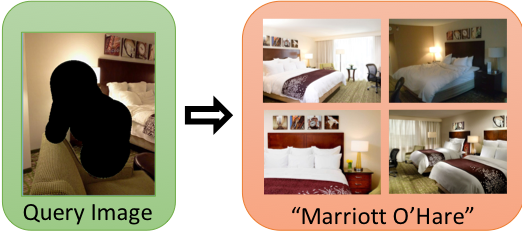
\includegraphics[width=.7\columnwidth]{figures/chapter1/victimQuery_to_hotel.png}
    \caption{The task of hotel recognition in cases of human trafficking involves identifying the particular hotel from an image of a trafficking victim.}
    \label{fig:victimQuery_to_hotel}
\end{figure}

Figure~\ref{fig:victimQuery_to_hotel} shows an example image from investigators, where a victim is posed in a hotel room. The hotel recognition task is to identify what hotel the victim was photographed in. The properties of the victim photographs further complicate the hotel recognition task -- the images are often of low quality, from uncommon camera perspectives, with large occlusions (often the victim).

Developing hotel recognition algorithms that are robust to these difficult query conditions is not only an interesting computer vision challenge, but also has very real human impacts.

% this chapter should present how we're going to solve the hotel recognition problem and give the roadmap for the remaining parts of the document that focus on traffickcam. (1) train a deep learning network using publicly available travel images; (2) why we need the traffickcam app

\section{Deep Learning for Recognition Problems}
\todo{Add section w/ background and related work on scene recognition and image similarity; discuss treating this as an image similarity problem; introduce why we need TraffickCam as segue into Chapter 2}
The place recognition problem be formulated as an image retrieval task where images of known locations serve as a database, and a query image's location is inferred by finding visually similar images in the dataset~\cite{baatz2012large,chen2011city,crandall2009mapping,hays2008im2gps,jacobs07geolocate,schindler2007city,torii2013visual,zamir2010accurate,googleLandmarks}.

\todo{Discuss previous approaches w/ local features, since that's what our preliminary experiments in the AIPR paper does.}

Increasingly, however, state of the art approaches to place recognition involve training deep neural networks to produce similar features for images from nearby locations~\cite{zhou2014recognizing,netvlad,visualPlaceRecognition,vo2017revisit,zhai2018geotemporal}.

\todo{Explain that while we can use these off-the-shelf networks, and some even have classes like 'hotel room' or 'bedroom', we know that we want to train networks with tons of hotel room images and that in order to do domain transfer well to real world query images, we'll need images from more than just travel websites.}